\documentclass[10pt]{beamer}

\usepackage[english]{babel}
\usepackage[utf8]{inputenc}
\usepackage[T1]{fontenc}
\usepackage{lmodern}

%\usepackage{caption}
%\usepackage{subcaption}
\usepackage{layout}
%\usepackage{epsfig}
\usepackage{graphicx}
\graphicspath{{images/}}
\usepackage[outdir=images/]{epstopdf}
\usepackage{tikz}
\usepackage{numprint}
%\usepackage{subfigure}
\usepackage{caption}
\usepackage{subcaption}
\captionsetup{compatibility=false}


\usepackage{siunitx}
\usepackage{eurosym}

\usepackage{amsthm}
\usepackage{amsmath}
\usepackage{amssymb}

\usepackage{mathrsfs}
\usepackage{wrapfig}
\usepackage{url}
\usepackage{multirow}
\usepackage{array}
\usepackage{pgfplots}

\usepackage[version=3]{mhchem}

\usepackage{wasysym}
%Bibtex
%\usepackage[square]{natbib}
%\newcommand{\newblock}{}

\usetheme{Warsaw}
\setbeamertemplate{headline}{}

%\usepackage{graphicx}
%\usepackage{epsfig}
%\usepackage{epstopdf}

\makeatletter
\newcommand*{\rom}[1]{\expandafter\@slowromancap\romannumeral #1@}
\makeatother

\usepackage{todonotes}
\title{Multi-characteristics reputation system using iterative filtering}
\author[Malian DR, Quentin L]{
  \small
  Malian De Ron
 \and
  Quentin Laurent
}

\begin{document}

\begin{frame}
  \maketitle
\end{frame}

\begin{frame}[allowframebreaks]
\frametitle{Reminder}
\begin{block}{Tensors in use}
\centering
\begin{tabular}{@{}ccl@{}}
\hline
Tensor & Size                  & Definition                                                                                                     \\ \hline
$X$    & $N \times M \times K$ & $X_{ijk}$ is the evaluation given by rater i\\
          &                                     &  to object j on characteristic k. \\
$A$    & $N \times M \times K$ & The adjacency matrix. $A_{ijk} = 1$ if \\
          &                                & rater $i$ evaluates $j$ on characteristic $k$, \\
          &                                & otherwise $A_{ijk} = 0$. \\
$R$    & $M \times K$          & The reputation matrix of objects. \\
$w$    & $N \times 1$          & The weight vector.     \\
$m_i$ & $N \times 1$          & Sum of characteristics evaluated by i. \\                                                                                      
\end{tabular}
\end{block}

\framebreak

    \begin{block}{Two steps iteration with sparsity matrix}
    Update of the reputations and weights
        \[
            R_{jk}^{t+1}(w^t,X) = \frac{\sum_{i=1}^N X_{ijk}w^t_{i}}{\sum_{i=1}^{N} A_{ijk} w^t_{i}} \quad 
        	w_i^{t+1}(X,R) = 1 -k \cdot \mathrm{div}_i \]

    \end{block}
    
    
    \begin{block}{}
    Distance of votes of judge $i$ to the reputation of object $j$
    \[d^{ij}_k= X_{ijk}-A_{ijk}\cdot R^{t+1}_{jk} \]
    Belief divergence
    \[ \mathrm{div}_i =  \frac{1}{m_i}\sum_{j=1}^N (d^{ij})^T (d^{ij}) \qquad m_i = \sum_{j=1}^{N} \sum_{k=1}^{K} A_{ijk} \]
     %                           with $k$ a constant.
    \end{block}
    %The farther a judge $i$ rates from the reputation, the lesser its weight.
\end{frame}

\begin{frame}
\frametitle{Properties of the method}
\begin{block}{Energy function(case $X$ dense)}
\begin{itemize}
\item Fix points of the iteration are stationary points of the energy function
$$E(r) =  \sum_{i=1}^n \int_0^{div_i(r)}g(u) du + c $$with $g(u) = 1 -ku$
\item Minimizing the energy function corresponds to maximizing the $\| \cdot \|_2$ of the weights
$$E(r) = \sum_{i=1}^N div_i - k \frac{div_i^2}{2} + \frac{2N}{k} = \|w\|_2$$
\item The iteration corresponds to a steepest descent method step of this energy function
$$r^{t+1} = r^t - \alpha_t \nabla_r E(r^t)\text{, }\quad\text{ with }\alpha^t = \frac{MK}{2 \sum_{i=1}^N w^t_i}$$
\end{itemize}
\end{block}
\end{frame}
\begin{frame}
\frametitle{Properties of the method}
\framesubtitle{Uniqueness}
\begin{block}{Mexican hat}
Let the function $E(r) : \mathbb{R}^n \rightarrow \mathbb{R} : E(r) = z $ be a fourth-order polynomial and let $\mathcal{H}$ be some hypercube in $\mathbb{R}^n$. If 
$$\lim_{||r||\rightarrow \infty} E(r) = - \infty $$
and the steepest descent direction on the boundary of $\mathcal{H}$ points strictly inside $\mathcal{H}$, then $E$ has a unique stationary point in $\mathcal{H}$ which is a minimum.
\end{block}
\begin{figure}
\centering
\begin{subfigure}{0.5\textwidth}
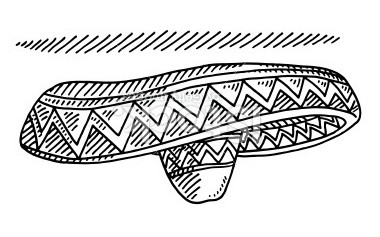
\includegraphics[width = 4cm]{mexicanhat.jpg} 
\end{subfigure}
\begin{subfigure}{0.49\textwidth}
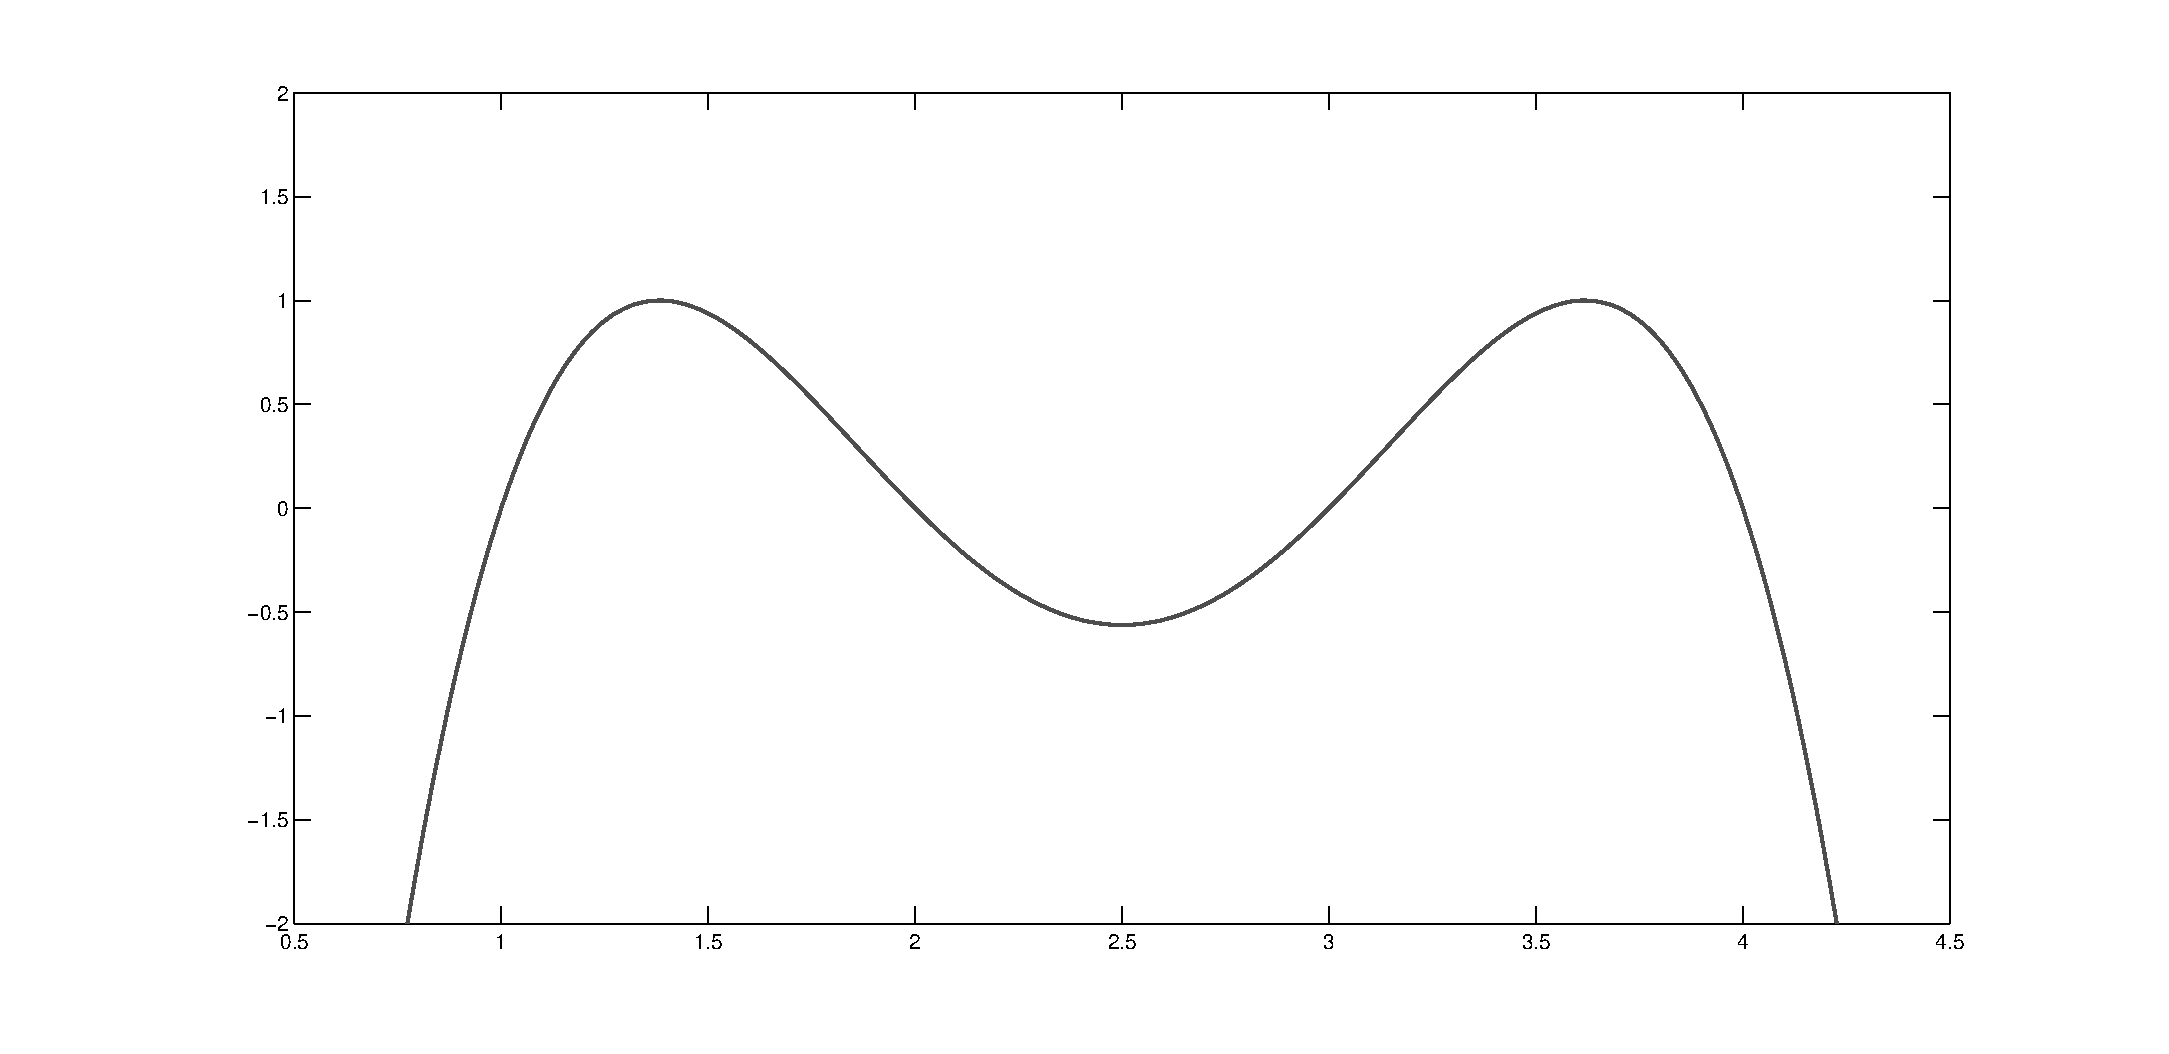
\includegraphics[width = 5cm]{mexicangraph.eps}
\end{subfigure}
\end{figure}
\begin{block}{}
If the weights are all positive, the system has a unique fixed point $r^{\star}$ in the domain.
\end{block}
\end{frame}

\begin{frame}
\frametitle{Influence of the parameter $k$}
\framesubtitle{Limitations}
\begin{block}{Domain for $k$}
\begin{itemize}
\item The greater the $k$, the more inconsistent judges will be penalized
\item The weights must be positive
$$k\in \mathcal{K} = \{k\in \mathcal{R}_{\geq 0} | 1 - k \begin{pmatrix} div_1 \\ div_2 \\ \vdots \\ div_n \end{pmatrix} >0 \: \forall r \in \mathcal{H} \}$$
\item In some cases, we would like to choose the highest $k$ possible
\end{itemize}
\end{block}

\end{frame}

\begin{frame}
\frametitle{Influence of the parameter $k$}
\framesubtitle{Modified method}
\begin{block}{Non-fixed $k$}
\begin{itemize}
\item Use of a sequence $k^t$
\item $k^t$ is such that at each iteration the weights are non-negative
$$ k^t : \min_i w_i^t = 0$$
%\item The sequence converges in general
\end{itemize}
\end{block}
\begin{block}{Shortcoming of the method}
\begin{itemize}
\item The greatest belief divergence limits the highest value of $k$.
\item Some cheaters with high belief divergence could shield other more subtle cheaters
\end{itemize}
\end{block}
\end{frame}


\begin{frame}{Reminder}
       
\end{frame}

\begin{frame}{Two steps iteration with sparsity matrix}

    \begin{block}{Reputation computation}
        \[
            R_{jk}^{t+1}(w^t,X) = \frac{\sum_{i=1}^N X_{ijk}w^t_{i}}{\sum_{i=1}^{N} A_{ijk} w^t_{i}}
        \]
    \end{block}
    Simple weighted sum of the votes.
    
    \begin{block}{Filtering}
                                \[ d^{ij}_k = X_{ijk}-A_{ijk} \cdot R^{t+1}_{jk} \]
                                \[ \mathrm{div}_i =  \frac{1}{m_i}\sum_{j=1}^N (d^{ij})^T (d^{ij}) \qquad m_i = \sum_{j=1}^{N} \sum_{k=1}^{K} A_{ijk}\]
                                \[ w_i^{t+1}(X,R) = 1 -k \cdot \mathrm{div}_i \]
                                with $k$ a constant.
    \end{block}
    The farther a judge $i$ rates from the reputation, the lesser its weight.
       
\end{frame}

\begin{frame}{Cheating}
        \begin{exampleblock}{Question}
            How does a cheater determine which value to give his ratings in order to maximize (or minimize) a final rating? He can't!
        \end{exampleblock}
        
        \begin{figure}
            \centering
            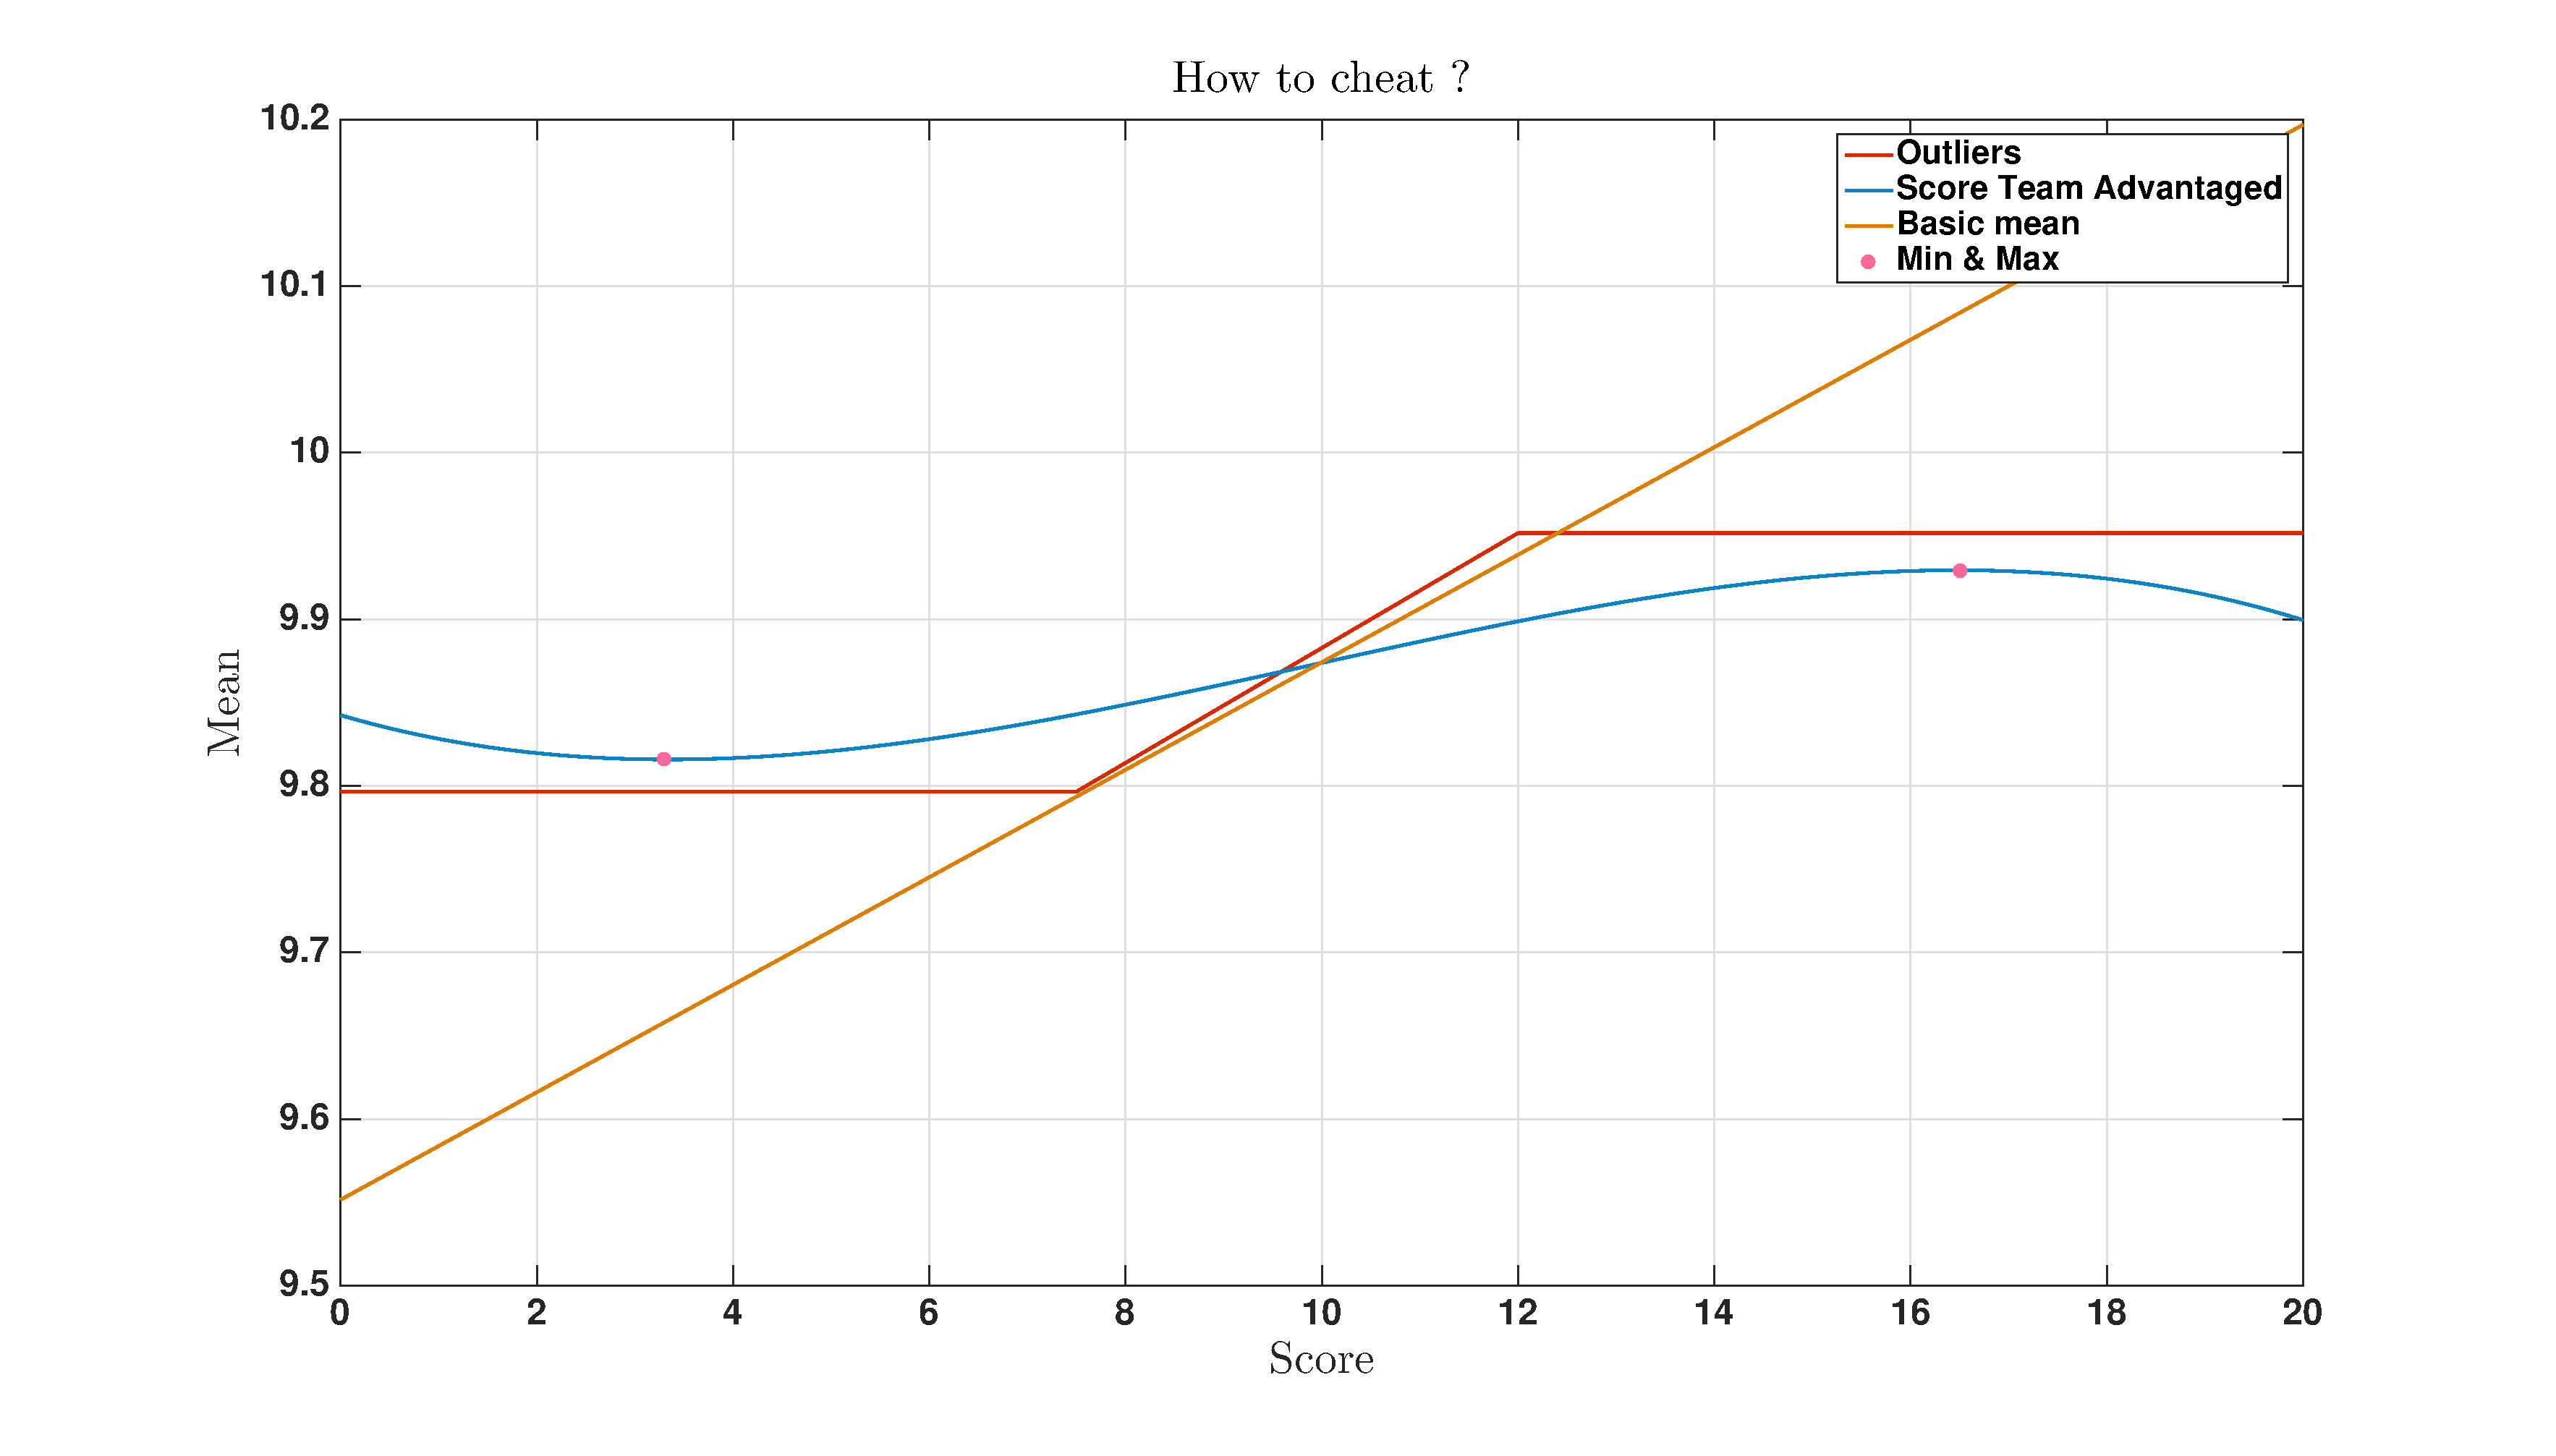
\includegraphics[width=\textwidth]{../rapport/images/cheaters/howto.eps}
        \end{figure}
\end{frame}

\begin{frame}{Application \rom{1}: MAP Scores}

\end{frame}

\usebackgroundtemplate{%
    \tikz\node[opacity=0.1] {
\includegraphics[height=\paperheight]{images/tripadvisor.jpg}};
}
\begin{frame}{Application \rom{2}: Hotels}
\begin{itemize}
    \item Subset of \textit{TripAdvisor}:
    \begin{itemize}
        \item \numprint{1 169 410} users
        \item \numprint{12 773} hotels
        \item \numprint{10} characteristics rated between 0 and 5\\ (service, cleanliness, price, location, $\dots$)
    \end{itemize}
    \item Preprocessing:
    \begin{itemize}
        \item[Step 1:] Keep only the users who voted for at least 4 hotels
        \item[Step 2:] Keep only the hotels that have at least 2 votes
        \item[Step 3:] If some users have only three votes or less, go to step 1
    \end{itemize}
    \item After preprocessing:
    \begin{itemize}
        \item \numprint{20 024} users
        \item \numprint{308} hotels
        \item \numprint{9} characteristics
    \end{itemize}
    \item Data are very sparse !
    \item Unfortunately, we do not detect a specific behaviour :(
\end{itemize}
\end{frame}

\begin{frame}{Application \rom{2}: Hotels with spammers (1)}
    Added 20 spammers giving always 0 except for their preferred hotel, which they rated 5 on all characteristics.
            \begin{figure}
            \centering
            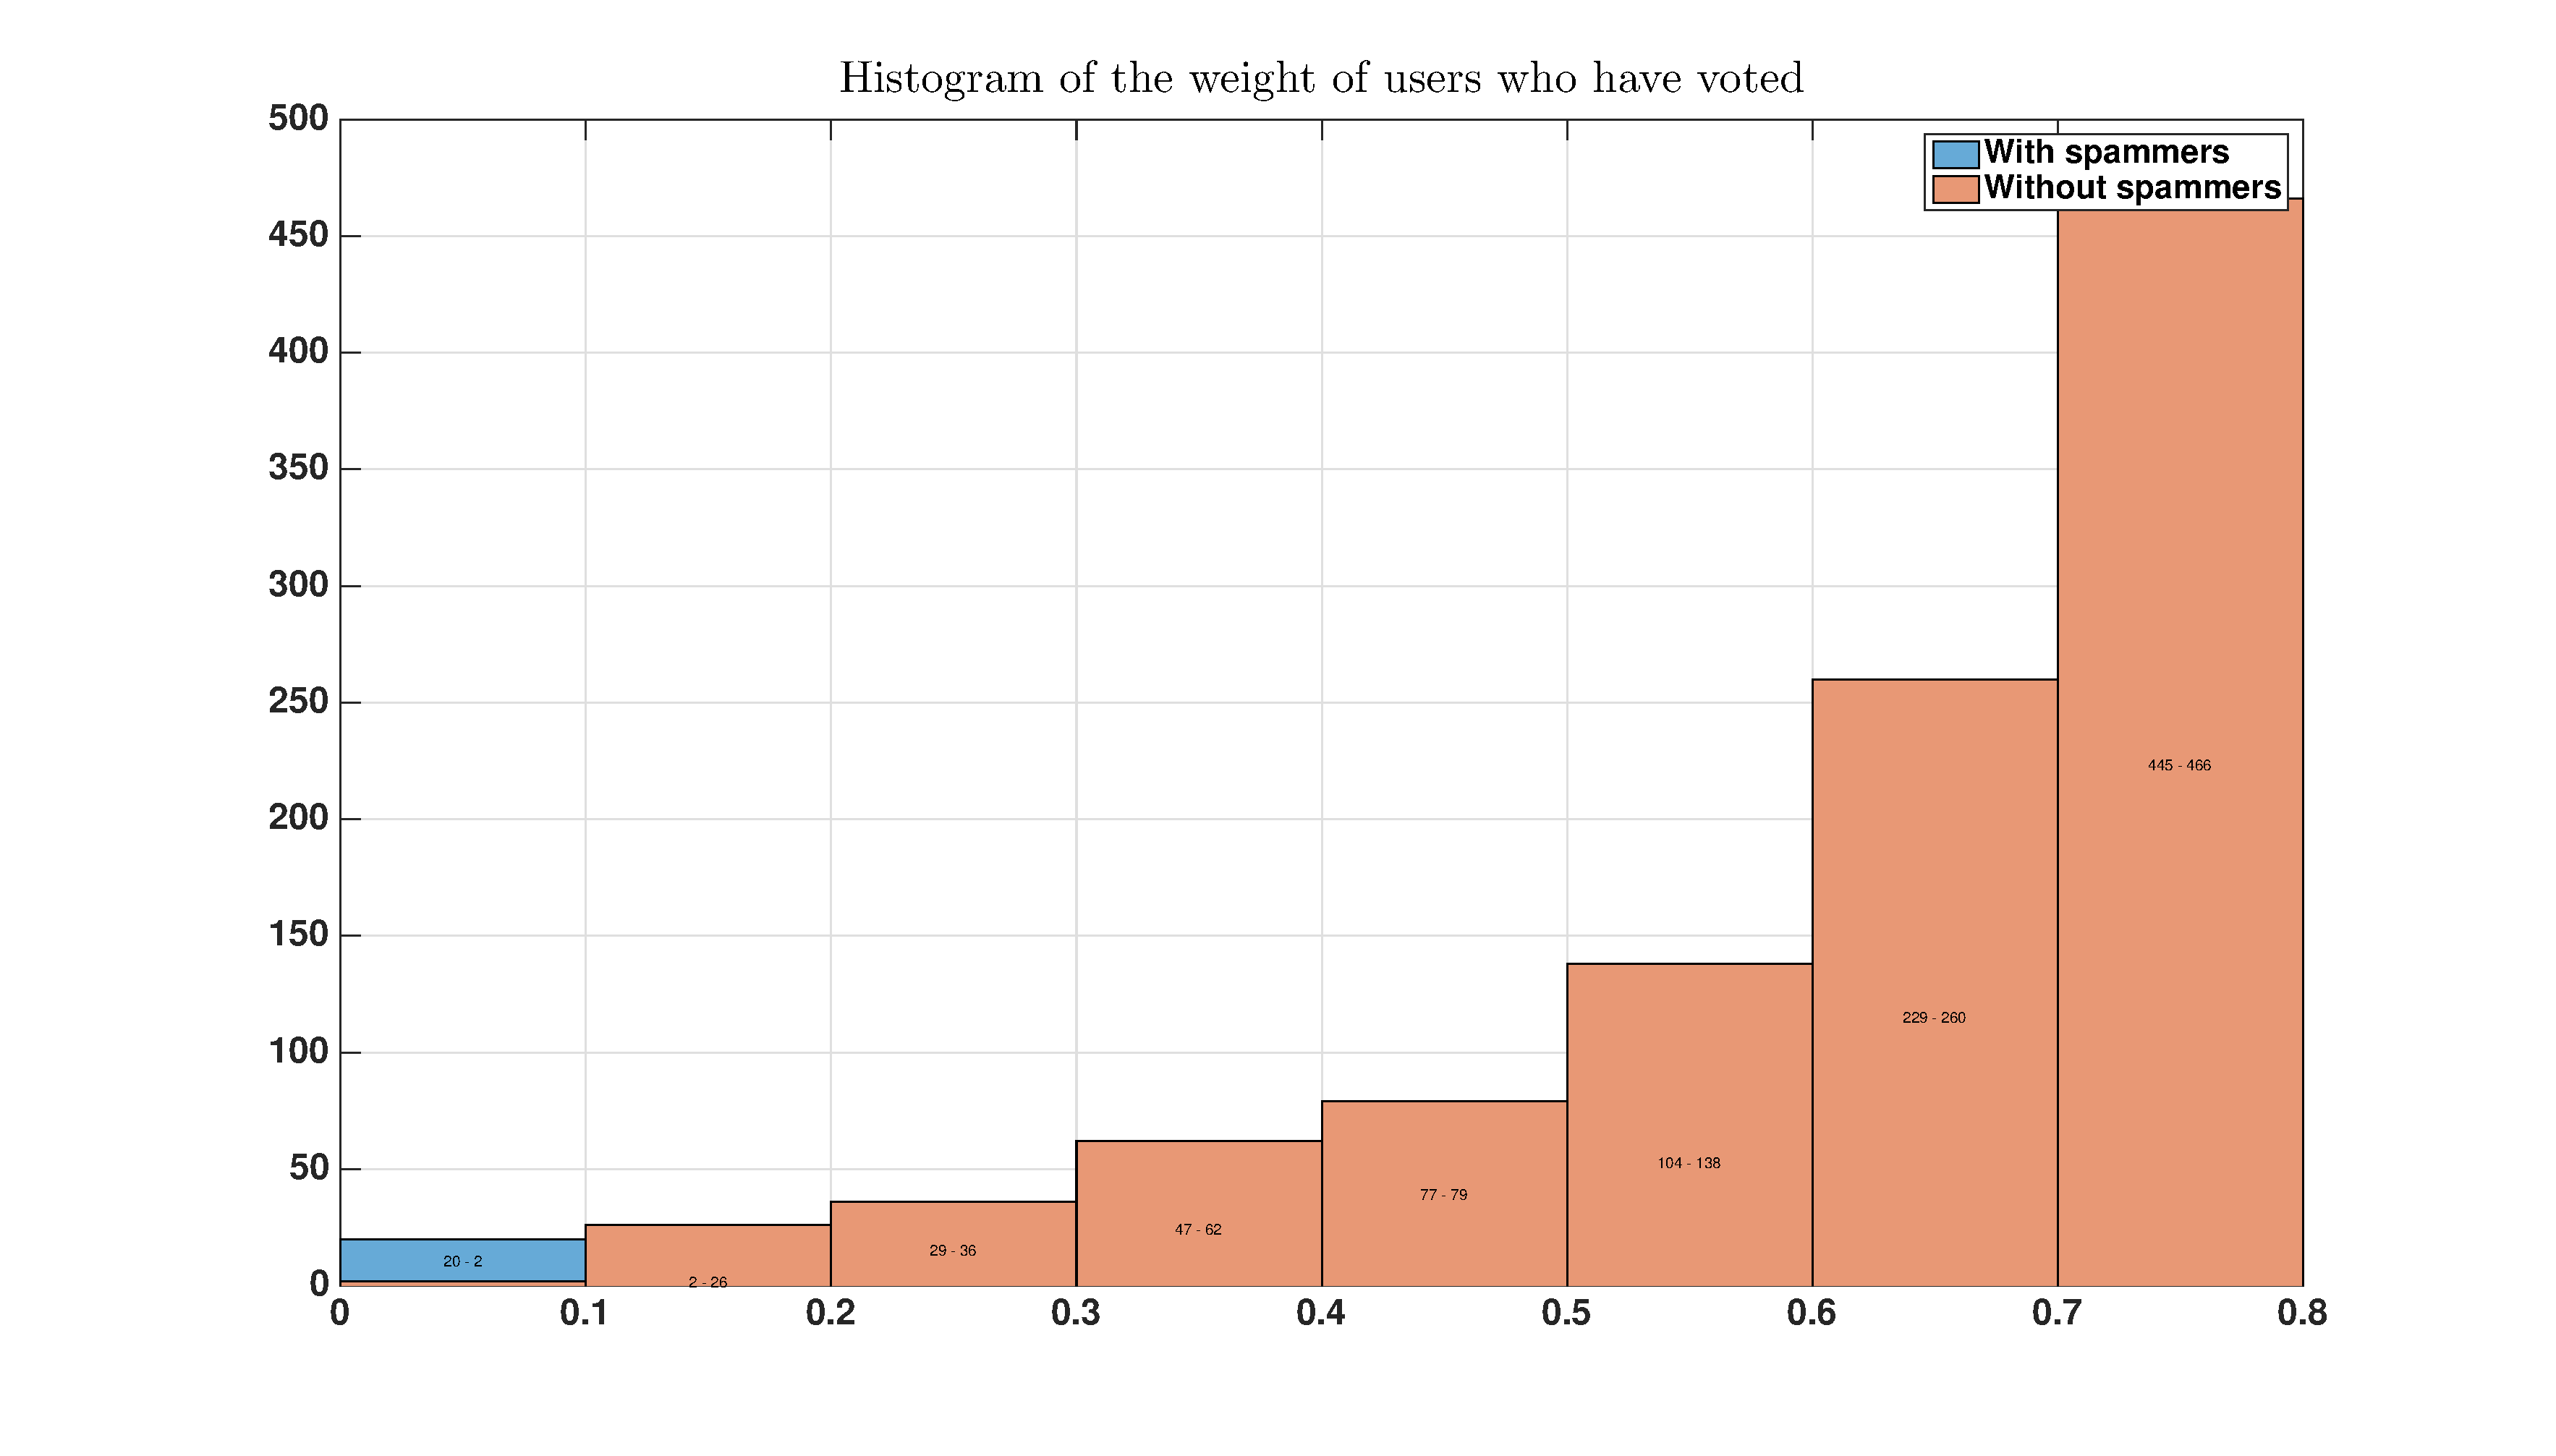
\includegraphics[width=\textwidth]{../rapport/images/hotels/not_random_cheaters.eps}
        \end{figure}
\end{frame}

\begin{frame}{Application \rom{2}: Hotels with spammers (2)}
    We now added to the original data set one spammer per hotel giving always 0 except for their own hotel, which they rated 5.
            \begin{figure}
            \centering
            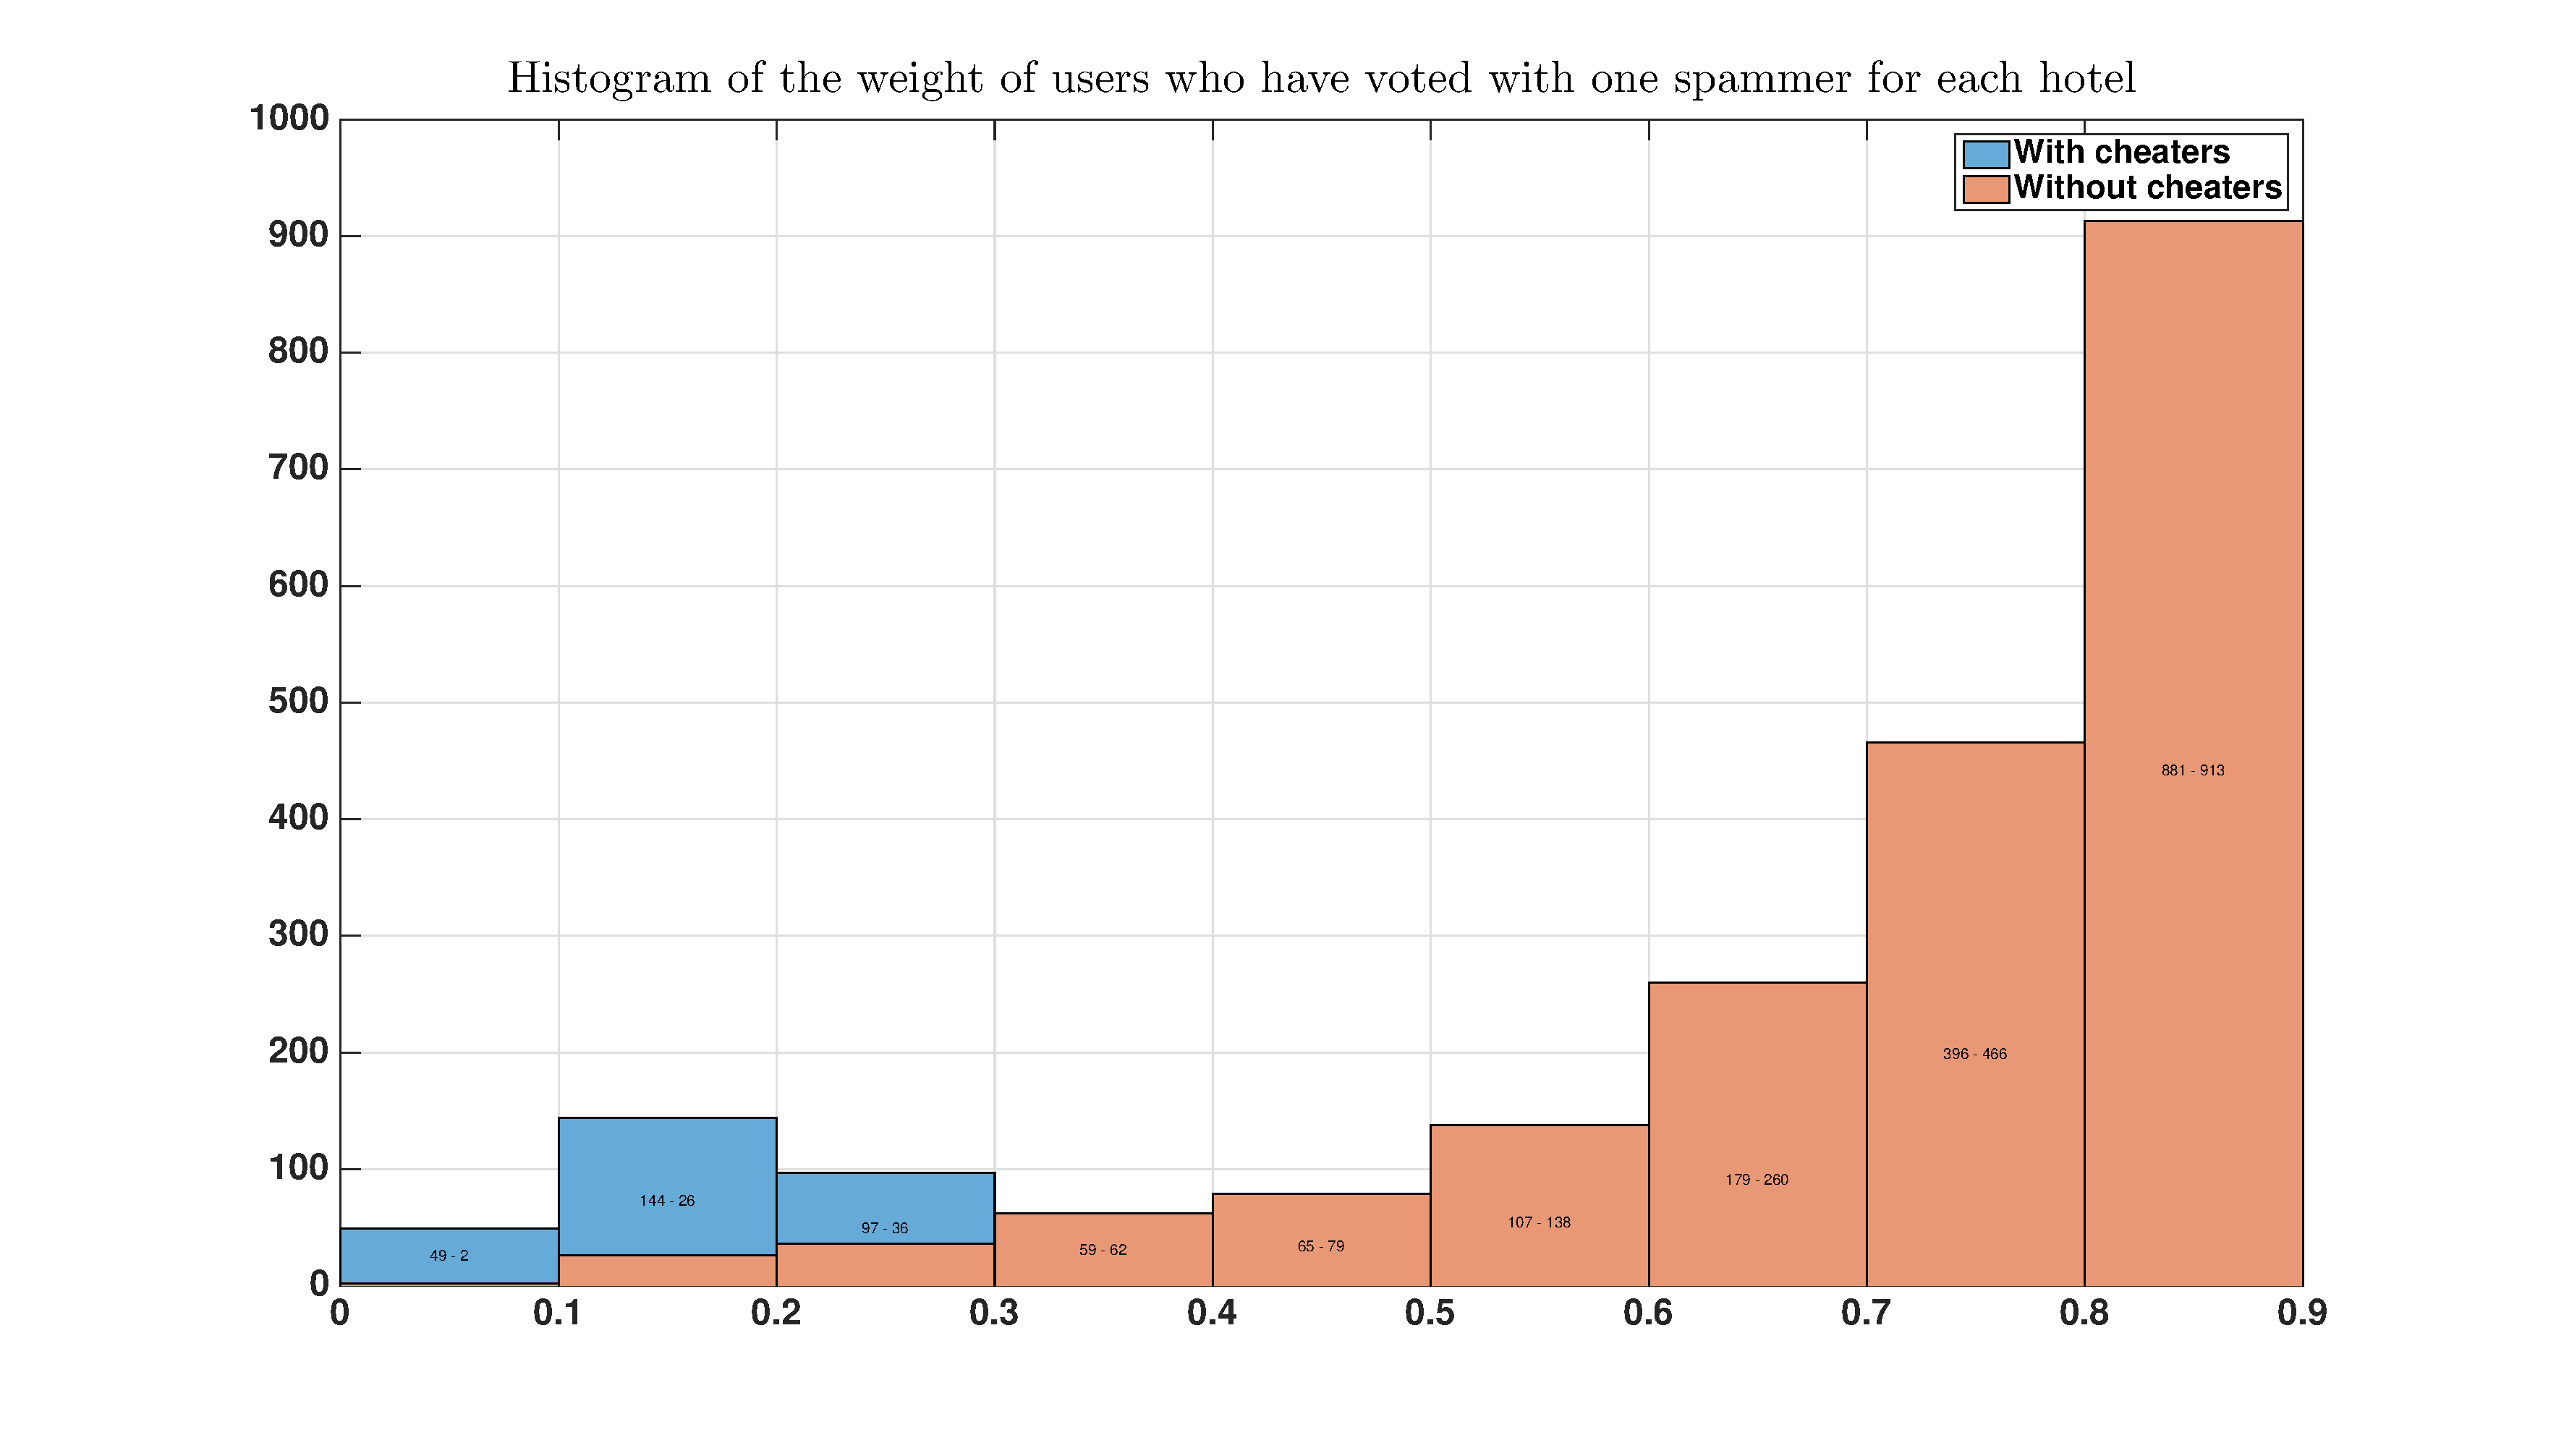
\includegraphics[width=\textwidth]{../rapport/images/hotels/not_random_each_hotels.eps}
        \end{figure}
\end{frame}

\begin{frame}{Conclusion}

\end{frame}



\end{document}
